Evaluating \acrshort{vo} is an important task. This section serves an overview of different ways for \acrshort{vo} evaluation and adopted in thesis scope. Furthermore, it evaluates results, observations and suggestions which may still improve existing result but unfortunately, they are not possible in this thesis due to time limit.
  
\section{Evaluation Criteria}
Evaluation can be of two types namely qualitative and quantitative. Quantitative evaluation requires ground truth. It generally measures accuracy of \acrshort{vo} and it uses matrices like \acrfull{ate} or \acrfull{rpe} \cite{7782863}. \acrshort{ate} refers to the \acrshort{rmse} between estimated trajectory and ground truth where as \acrshort{rpe} calculates error between all sub-trajectories of \acrshort{vo} and ground truth. Both matrices have their pros and cons like complexity, reliability etc. The qualitative approach includes Robustness of \acrshort{vo} in some conditions like motion blur, low texture (less features) scene, dynamic environment, scene brightness etc. Robustness defines the ability to recover the track (or finding loop closure in case of \acrshort{v-slam}) after loosing localization due to environment. Another approach includes efficiency factors like computation power, memory usage, processing speed etc. Not all criteria need to be fulfill and also not every \acrshort{vo} method can satisfy them rather it depends on application or use-cases that which criteria to use. Figure \ref{fig:matrices} shows how each evaluation criteria are different from each other for \acrshort{vo} methods.     
\begin{figure}[H]
	\centering
	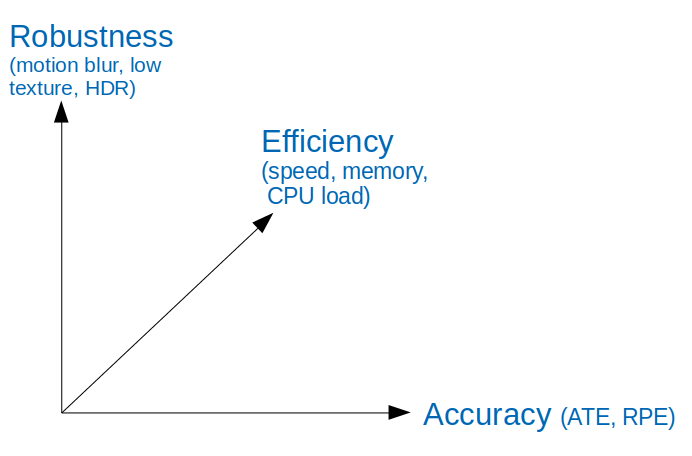
\includegraphics[width=.8\textwidth]{matrices}
	\caption{Different matrices for \acrshort{vo} evaluation \cite{lecture}}
	\label{fig:matrices}
\end{figure}

\section{Experiment}
This section describes result of all the offline measurements taken during data acquisition step. Every measurement is run in total seven times because it contains both cameras and also \acrshort{lidar} raw data and tested on four odometry algorithms i.e. three \acrshort{vo} and one \acrshort{lidar} odometry. \acrshort{orb}-\acrshort{slam} and \acrshort{ldso} have visualization functionality implemented with them while \acrshort{svo} does not have this feature. An attempt is made to visualization using open-source software package Pangolin viewer but it is not successful and abandoned due to time limitation and non-priority. Therefore, in case of \acrshort{svo} and \acrshort{lidar} only trajectory plot can be made. Next subsections illustrate the experiment results of the data recorded during data acquisition step.

\subsection{Straight Path}
This measurement is taken nearly on the straight path consisting no rotations. Robot has little amount of drift in right wheel which is up to acceptable limit. Nearly 16 meter long path which took around 30 seconds. The total frames and keyframes detected in \acrshort{orb}-\acrshort{slam} and \acrshort{ldso} are given in table \ref{table:straight} and the trajectory of both camera is given in figure \ref{fig:Pico1} and \ref{fig:Web1}. for straight path the initialization was nearly same in both methods but longer for Genius widecam. \acrshort{svo} has very poor performance in all the experiment therefore its trajectory is not shown in any experiment. In case of \acrshort{orb}-\acrshort{slam}, the green and blue rectangles show current camera and previous cameras (trajectory) respectively. The red points describe the 3D local mapping. While in \acrshort{ldso} red rectangle is current camera and blue ones are active keyframes which are around 7 all the time. The yellow line depicts the camera trajectory and black points are the 3D map points.\\
\begin{table}[H]
	\centering
	\renewcommand{\arraystretch}{1.5}
	\begin{tabular}{ l| l| l |l }
		\textbf{Camera} & \textbf{Frames} & \multicolumn{2}{c}{\textbf{Keyframes}}  \\    
		&      & \textbf{Orb-Slam}  & \textbf{Ldso}  \\
		\hline
		Picocam & 446 &  41  & 105 \\ 
		\hline
		Genius F100 & 856 &  64  & 114 \\ 
	\end{tabular}
	\caption{Image frame details of Straight path}
	\label{table:straight}
\end{table}
\begin{figure}[H]
	\begin{subfigure}{.5\textwidth}
		\centering
		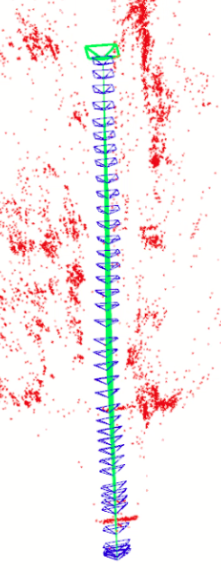
\includegraphics[width=0.5\linewidth]{orb_pico1}
		\caption{\acrshort{orb}-\acrshort{slam} trajectory}
		\label{fig:orb_pico1}
	\end{subfigure}%
	\begin{subfigure}{.5\textwidth}
		\centering
		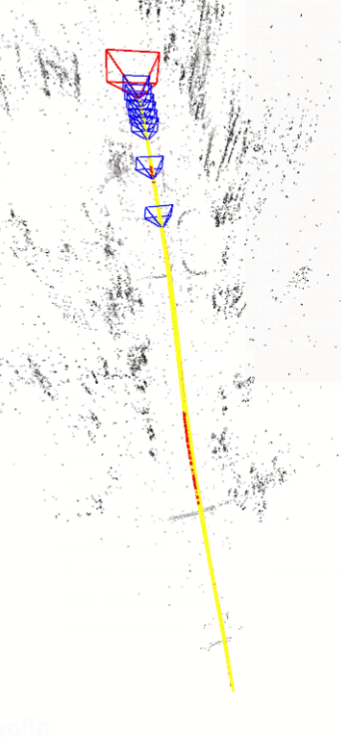
\includegraphics[width=0.5\linewidth]{ldso_pico1}
		\caption{\acrshort{ldso} trajectory}
		\label{fig:ldso_pico1}
	\end{subfigure}
	\caption{Picocam trajectories of straight path}
	\label{fig:Pico1}
\end{figure}
\begin{figure}[H]
	\begin{subfigure}{.5\textwidth}
		\centering
		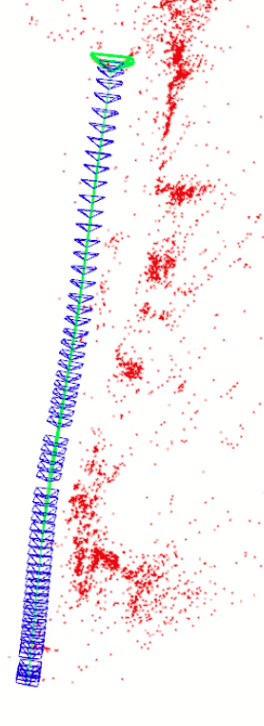
\includegraphics[width=.5\linewidth]{orb_web1}
		\caption{\acrshort{orb}-\acrshort{slam} trajectory}
		\label{fig:orb_web1}
	\end{subfigure}%
	\begin{subfigure}{.5\textwidth}
		\centering
		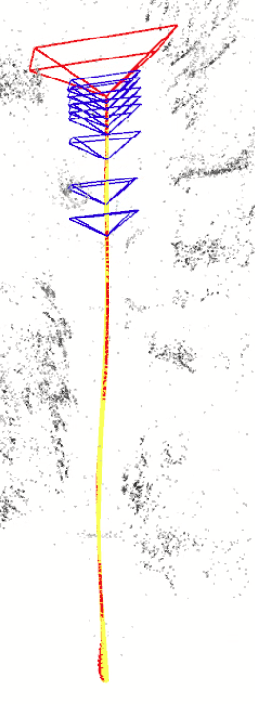
\includegraphics[width=.5\linewidth]{ldso_web1}
		\caption{\acrshort{ldso} trajectory}
		\label{fig:ldso_web1}
	\end{subfigure}
	\caption{Genius Widecam F100 trajectories of straight path}
	\label{fig:Web1}
\end{figure}

\subsection{Rectangle Path}
This recording is taken to analyse the drift in all methods without using loop closing functionality. The measurement start and ends at one point consisting no loop. Approximate length of rectangle is 8 m and width is 2 m. The table \ref{table:rectangle} shows details of keyframes and figures \ref{fig:Pico2} and \ref{fig:Web2} show camera trajectory tracked. It can be seen that only combination of \acrshort{orb}-\acrshort{slam} and Picocam gives satisfactory result where as \acrshort{ldso}  struggles to find the scene depth after two rotations and can not retrieve it. Also \acrshort{orb}-\acrshort{slam} with Genius Widecam can not perform well and lost the tracking after second rotation due to possible motion blur.
\begin{table}[H]
	\centering
	\renewcommand{\arraystretch}{1.5}
	\begin{tabular}{ l| l| l |l }
		\textbf{Camera} & \textbf{Frames} & \multicolumn{2}{c}{\textbf{Keyframes}}  \\    
		&      & \textbf{Orb-Slam}  & \textbf{Ldso}  \\
		\hline
		Picocam & 1090 &  91  & 218 \\ 
		\hline
		Genius F100 & 2042 &  38  & 209 \\ 
	\end{tabular}
	\caption{Image frame details of Rectangular path}
	\label{table:rectangle}
\end{table}
\begin{figure}[H]
	\begin{subfigure}{.6\textwidth}
		\centering
		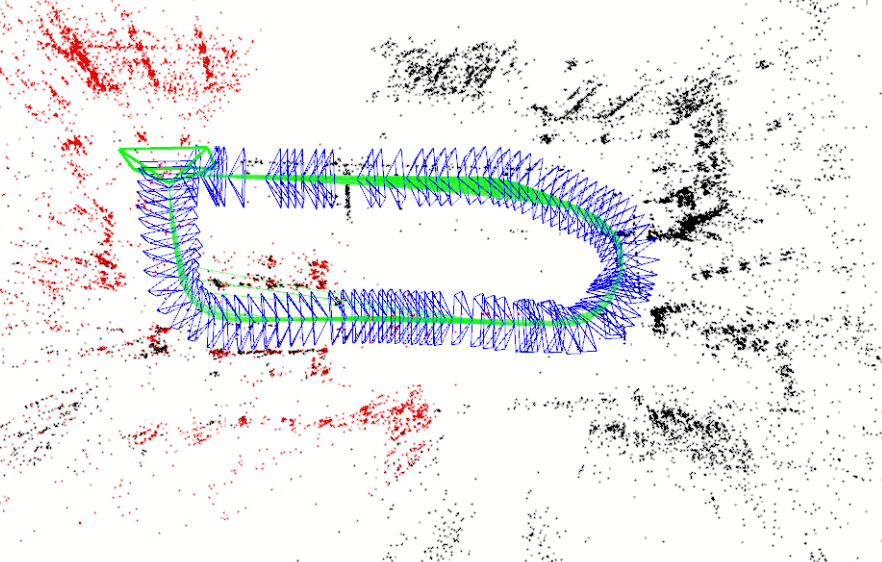
\includegraphics[width=1.0\linewidth]{orb_pico2}
		\caption{\acrshort{orb}-\acrshort{slam} trajectory}
		\label{fig:orb_pico2}
	\end{subfigure}
	\begin{subfigure}{.4\textwidth}
		\centering
		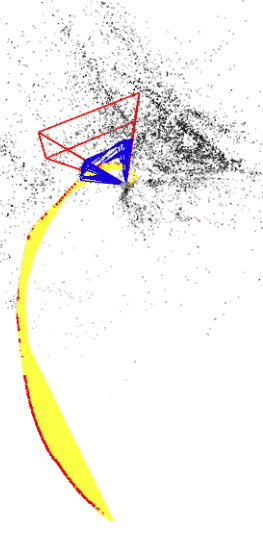
\includegraphics[width=0.8\linewidth]{ldso_pico2}
		\caption{\acrshort{ldso} trajectory}
		\label{fig:ldso_pico2}
	\end{subfigure}
	\caption{Picocam trajectories of rectangle path}
	\label{fig:Pico2}
\end{figure}
\begin{figure}[H]
	\begin{subfigure}{.6\textwidth}
		\centering
		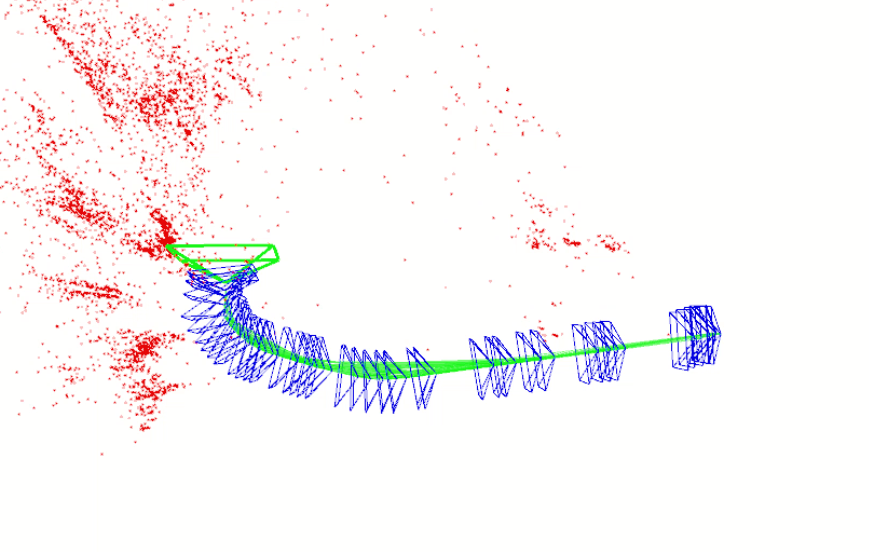
\includegraphics[width=1.0\linewidth]{orb_web2}
		\caption{\acrshort{orb}-\acrshort{slam} trajectory}
		\label{fig:orb_web2}
	\end{subfigure}%
	\begin{subfigure}{.4\textwidth}
		\centering
		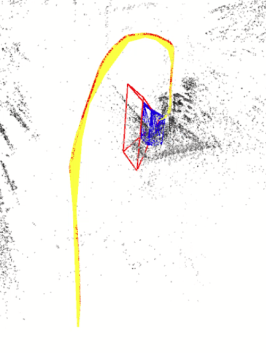
\includegraphics[width=.9\linewidth]{ldso_web2}
		\caption{\acrshort{ldso} trajectory}
		\label{fig:ldso_web2}
	\end{subfigure}
	\caption{Genius Widecam F100 trajectories of rectangle path}
	\label{fig:Web2}
\end{figure}

\subsection{Repeated Path}
This measurement consist one loop with same path. The frames details can be seen in \ref{table:repeated}. Here also the combination of \acrshort{orb}-\acrshort{slam} and Picocam is clear winner as seen in figures \ref{fig:Pico3} and \ref{fig:Web3}. \acrshort{ldso} can also detect multiple loops (four) in both cameras and even performs better in case of Genius Widecam than that of Picocam but cannot outperform \acrshort{orb}-\acrshort{slam}. A main reason is that this experiment has many rotations which is not so good for \acrshort{ldso}. It starts drifting as more rotations come in to picture.\\
\begin{table}[H]
	\centering
	\renewcommand{\arraystretch}{1.5}
	\begin{tabular}{ l| l| l |l }
		\textbf{Camera} & \textbf{Frames} & \multicolumn{2}{c}{\textbf{Keyframes}}  \\    
		&      & \textbf{Orb-Slam}  & \textbf{Ldso}  \\
		\hline
		Picocam & 1432 &  120  & 591 \\ 
		\hline
		Genius F100 & 2373 &  176  & 440 \\ 
	\end{tabular}
	\caption{Image frame details of Repeated path}
	\label{table:repeated}
\end{table}
\begin{figure}[H]
	\begin{subfigure}{.5\textwidth}
		\centering
		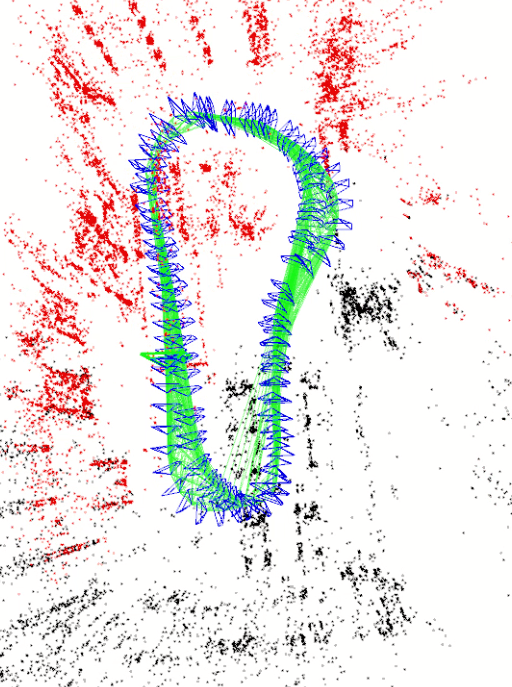
\includegraphics[width=1.0\linewidth]{orb_pico3}
		\caption{\acrshort{orb}-\acrshort{slam} trajectory}
		\label{fig:orb_pico3}
	\end{subfigure}
	\begin{subfigure}{.5\textwidth}
		\centering
		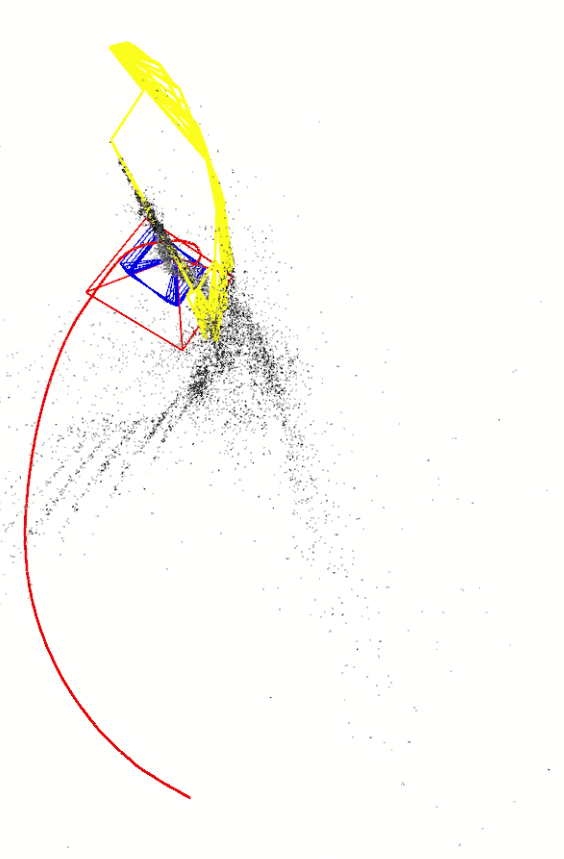
\includegraphics[width=0.8\linewidth]{ldso_pico3}
		\caption{\acrshort{ldso} trajectory}
		\label{fig:ldso_pico3}
	\end{subfigure}
	\caption{Picocam trajectories of repeated path}
	\label{fig:Pico3}
\end{figure}
\begin{figure}[H]
	\begin{subfigure}{.5\textwidth}
		\centering
		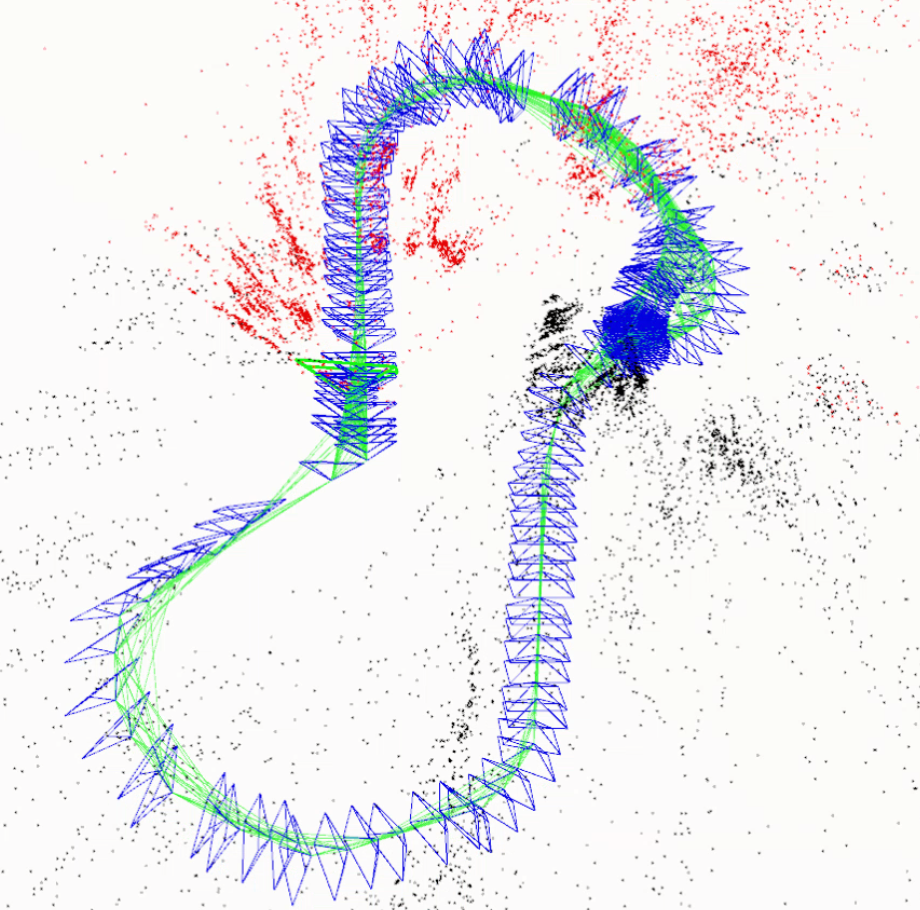
\includegraphics[width=1.0\linewidth]{orb_web3}
		\caption{\acrshort{orb}-\acrshort{slam} trajectory}
		\label{fig:orb_web3}
	\end{subfigure}%
	\begin{subfigure}{.5\textwidth}
		\centering
		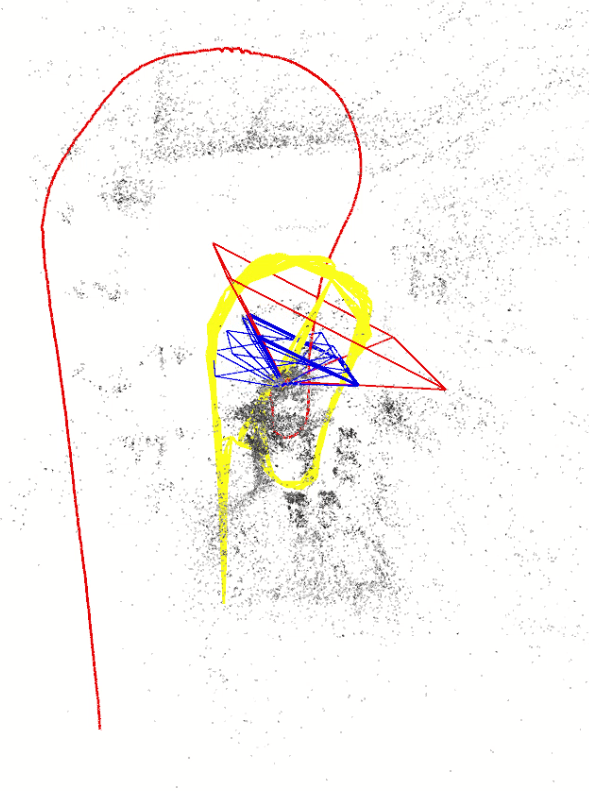
\includegraphics[width=1.0\linewidth]{ldso_web3}
		\caption{\acrshort{ldso} trajectory}
		\label{fig:ldso_web3}
	\end{subfigure}
	\caption{Genius Widecam F100 trajectories of repeated path}
	\label{fig:Web3}
\end{figure}

\subsection{Multi-loop Path}
This recording is longest in all experiments and contains multi-loops. \acrshort{ldso} cannot handle of this length of measurement due to high memory consumption and on Ubuntu PC-18.04 with 16 GB memory was not sufficient for it. Only \acrshort{orb}-\acrshort{slam} with Picocam can performed well for this data set as seen in figure \ref{fig:orb_pico4}. Total 6 times loops are detected. Number of keyframes tracked compared to total frames can be seen in table \ref{table:multi-loop}. It shows superiority of \acrshort{orb}-\acrshort{slam} than other \acrshort{vo} methods. At some location track is lost but as soon as a loop is detected the camera relocalizes and further improves pose optimization. 
\begin{table}[H]
	\centering
	\renewcommand{\arraystretch}{1.5}
	\begin{tabular}{ l| l| l |l }
		\textbf{Camera} & \textbf{Frames} & \multicolumn{2}{c}{\textbf{Keyframes}}  \\    
		&      & \textbf{Orb-Slam}  & \textbf{Ldso}  \\
		\hline
		Picocam & 3351 & 320   & - \\ 
		\hline
		Genius F100 & 6129  &  391  & - \\ 
	\end{tabular}
	\caption{Image frame details of Multi-loop path}
	\label{table:multi-loop}
\end{table}

\begin{figure}[H]
	\centering
	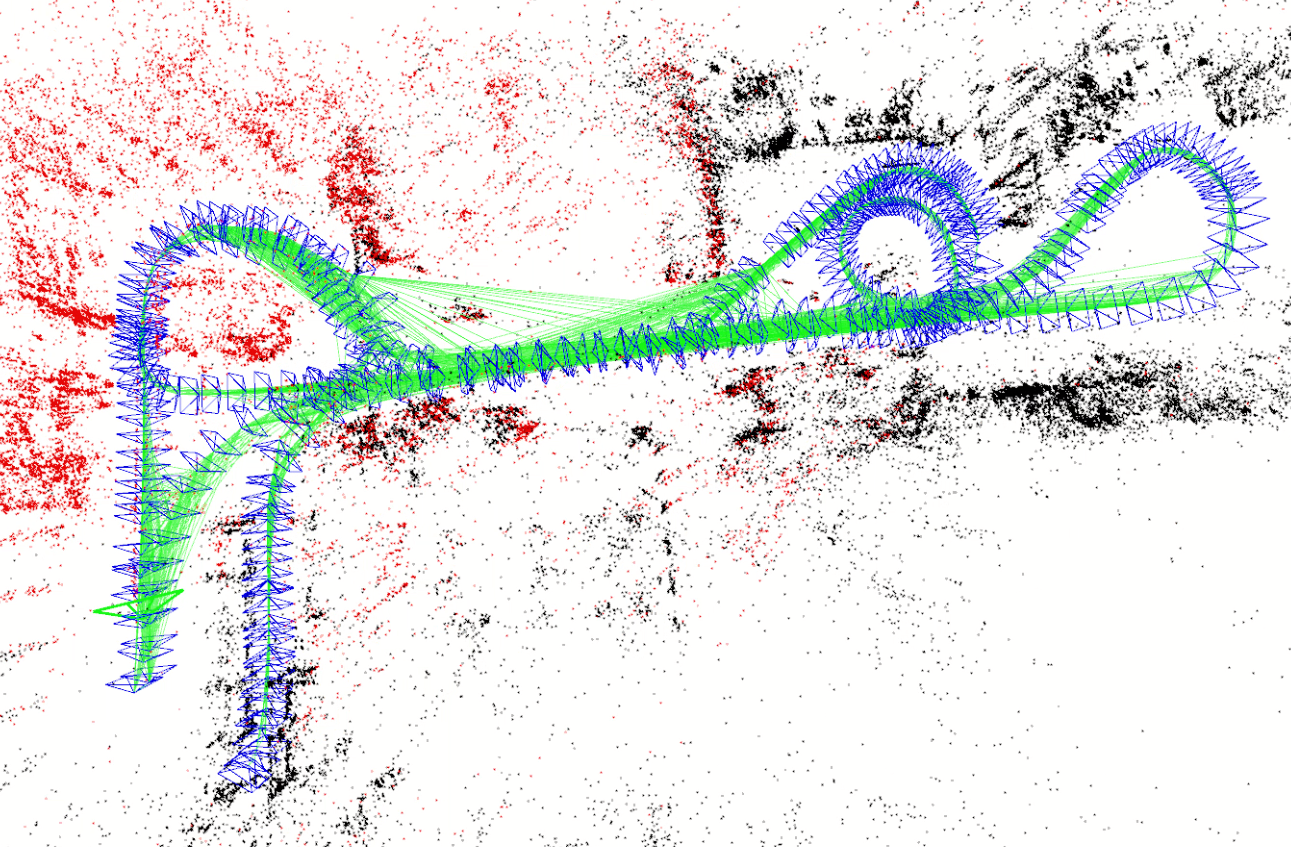
\includegraphics[width=1.0\linewidth]{orb_pico4}
	\caption{\acrshort{orb}-\acrshort{slam} trajectory}
	\label{fig:orb_pico4}
\end{figure}

\subsection{Figure Eight Path}
This data set contains many rotations and is used to evaluate the performance of \acrshort{vo} methods in this condition. As expected \acrshort{orb}-\acrshort{slam} performs very well in this case detecting many loops. Though \acrshort{ldso} detects many loops and takes more keyframes as shown in table \ref{table:eight} than \acrshort{orb}-\acrshort{slam} it has not ability to recover the motion after some rotations. This situation can be seen in figure \ref{fig:Pico5}. In case of Genius Widecam \acrshort{orb}-\acrshort{slam} starts drifting after starting rotation and which creates some motion blur and it relocalizes again when a loop is detected but it looses track at same location every time (see figure \ref{fig:orb_web5}). While in case of \acrshort{ldso} it works for a while but pose graph optimization does not work accurately and a symmetric pattern in figure eight can be obtained as in case of \acrshort{orb}-\acrshort{slam}.\\
\begin{table}[H]
	\centering
	\renewcommand{\arraystretch}{1.5}
	\begin{tabular}{ l| l| l |l }
		\textbf{Camera} & \textbf{Frames} & \multicolumn{2}{c}{\textbf{Keyframes}}  \\    
		&      & \textbf{Orb-Slam}  & \textbf{Ldso}  \\
		\hline
		Picocam & 1224 &  116  & 557 \\ 
		\hline
		Genius F100 & 2175 &  152  & 532 \\ 
	\end{tabular}
	\caption{Image frame details of figure eight path}
	\label{table:eight}
\end{table}

\begin{figure}[H]
	\begin{subfigure}{.5\textwidth}
		\centering
		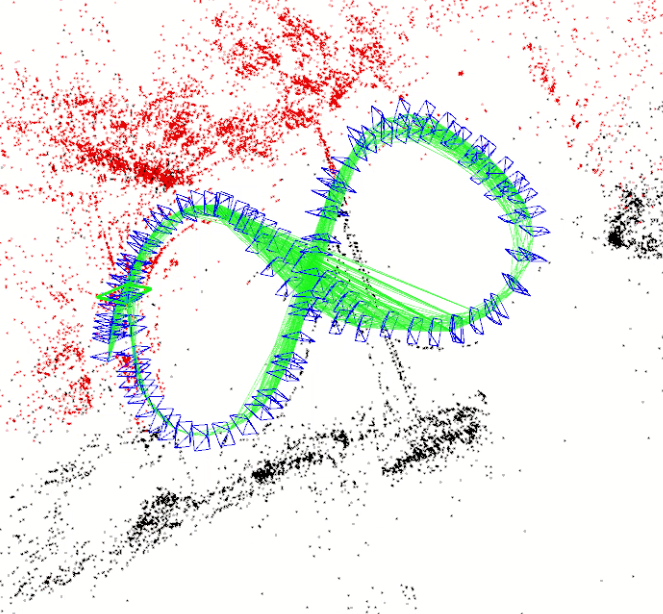
\includegraphics[width=1.0\linewidth]{orb_pico5}
		\caption{\acrshort{orb}-\acrshort{slam} trajectory}
		\label{fig:orb_pico5}
	\end{subfigure}
	\begin{subfigure}{.5\textwidth}
		\centering
		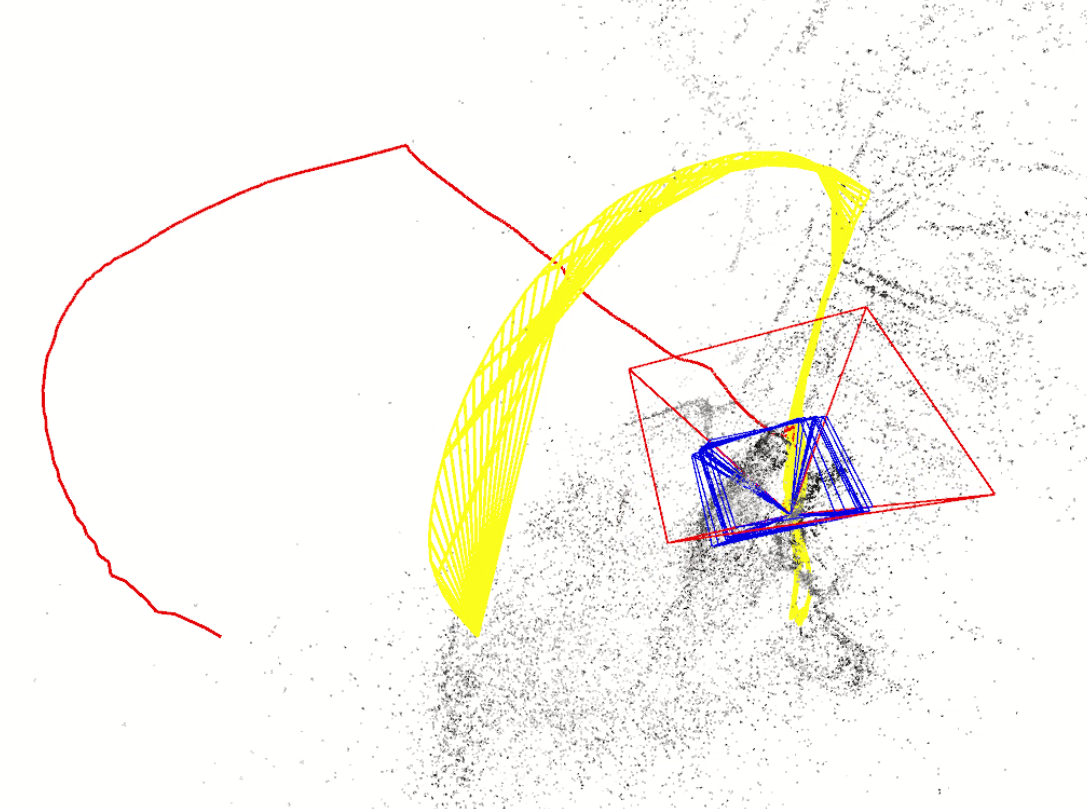
\includegraphics[width=1.0\linewidth]{ldso_pico5}
		\caption{\acrshort{ldso} trajectory}
		\label{fig:ldso_pico5}
	\end{subfigure}
	\caption{Picocam trajectories of figure eight path}
	\label{fig:Pico5}
\end{figure}
\begin{figure}[H]
	\begin{subfigure}{.5\textwidth}
		\centering
		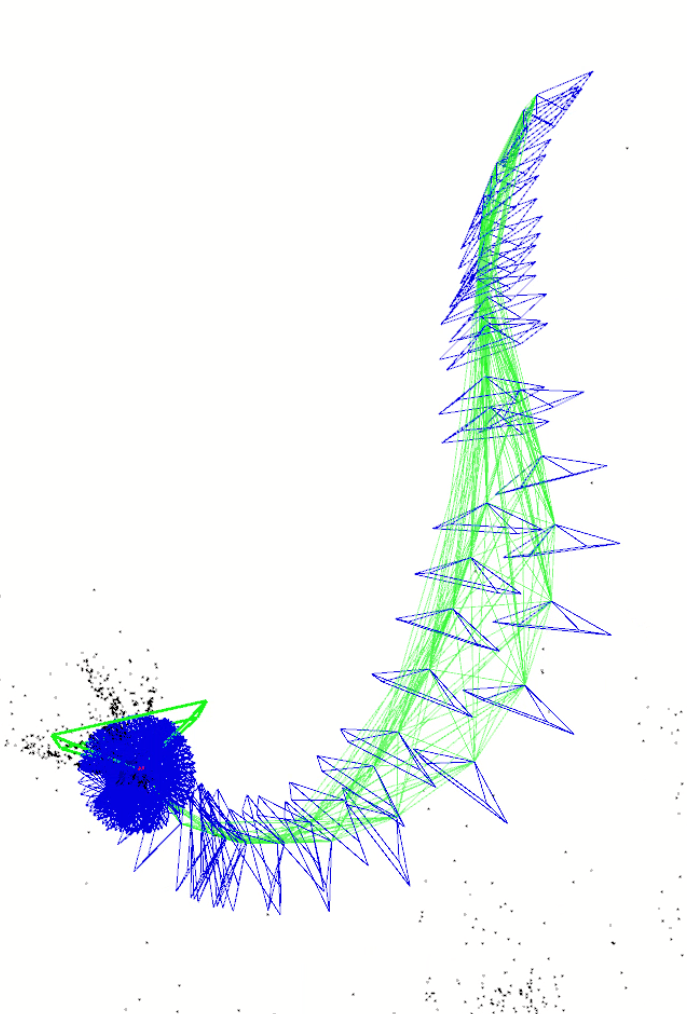
\includegraphics[width=1.0\textwidth]{orb_web5}
		\caption{\acrshort{orb}-\acrshort{slam} trajectory}
		\label{fig:orb_web5}
	\end{subfigure}%
	\begin{subfigure}{.5\textwidth}
		\centering
		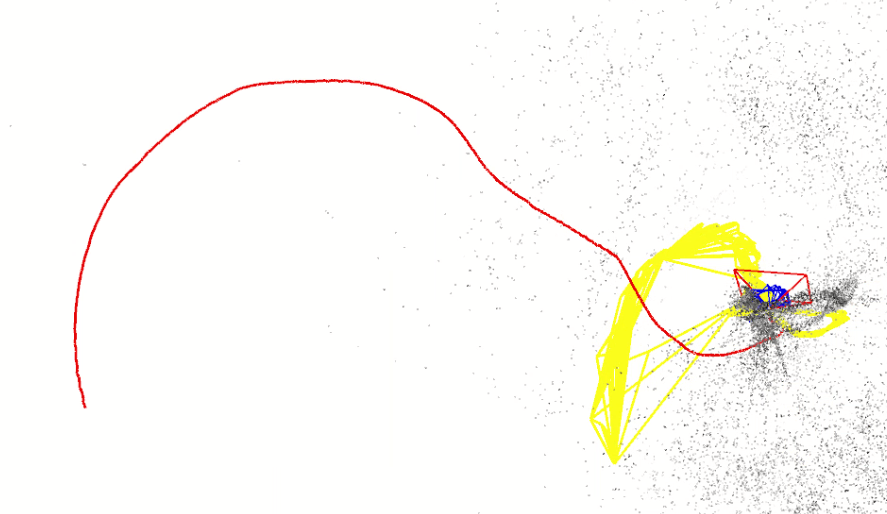
\includegraphics[width=1.0\linewidth]{ldso_web5}
		\caption{\acrshort{ldso} trajectory}
		\label{fig:ldso_web5}
	\end{subfigure}
	\caption{Genius Widecam F100 trajectories of figure eight path}
	\label{fig:Web5}
\end{figure}

\section{Comparison}
Due to scale ambiguity, monocular \acrshort{vo} can not be evaluated directly with ground truth or with \acrshort{lidar} odometry. The implementation of finding absolute scale is not successful. It is not possible to compute the accuracy of every \acrshort{vo} and compare them therefore qualitative approach is the only which can used as comparison. As described in experiment section \acrshort{svo} could not perform on any data sets. Furthermore, \acrshort{ldso} is also not performing well considering rotations and low brightness area. The only possible choice to compare with \acrshort{lidar} odometry is \acrshort{orb}-\acrshort{slam}. Picocam camera performance is always superior to Genius Widecam F100. Figure \ref{fig:straight} illustrates the comparison of \acrshort{lidar} odometry, \acrshort{orb}-\acrshort{slam} and \acrshort{ldso} trajectory (Picocam) on a straight path with known length of 16m without scale \ref{fig:straight1} and with a scale factor \ref{fig:straight2} of 4.8 (\acrshort{ldso}) and 6.0(\acrshort{orb}-\acrshort{slam}). Figure \ref{fig:rectangle} shows the trajectory comparison on rectangle path consisting no loop and same starting and goal position.   
\begin{figure}[H]
	\begin{subfigure}{.5\textwidth}
		%\centering
		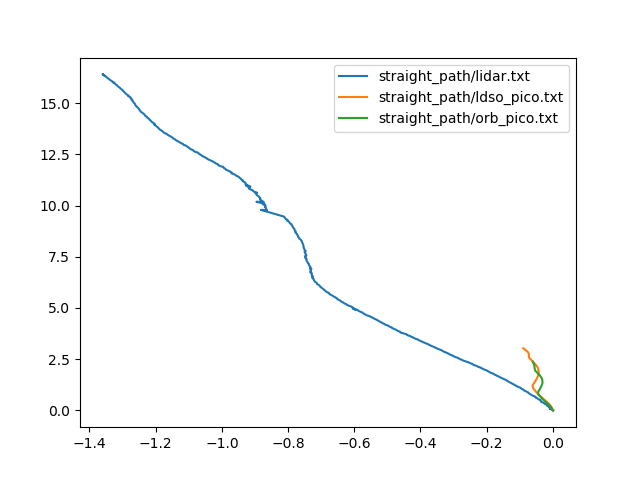
\includegraphics[width=1.0\linewidth]{straight1}
		\caption{Trajectory plot without scale factor}
		\label{fig:straight1}
	\end{subfigure}
	\begin{subfigure}{.5\textwidth}
		%\centering
		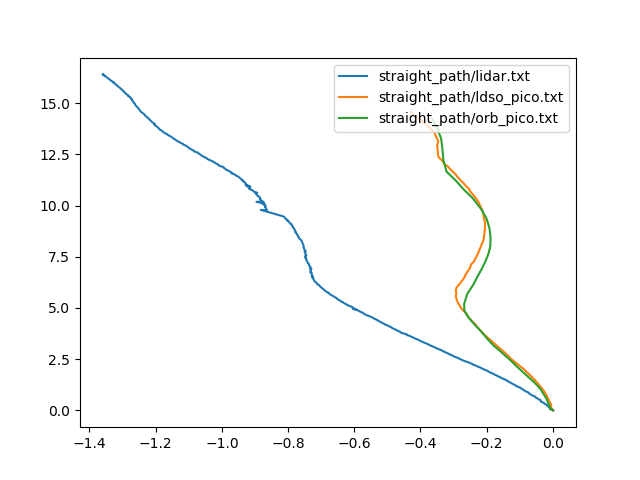
\includegraphics[width=1.0\linewidth]{straight2}
		\caption{Trajectory plot with scale factor}
		\label{fig:straight2}
	\end{subfigure}
	\caption{Trajectory plots of straight path}
	\label{fig:straight}
\end{figure}

\begin{figure}[H]
	\begin{subfigure}{.5\textwidth}
		%\centering
		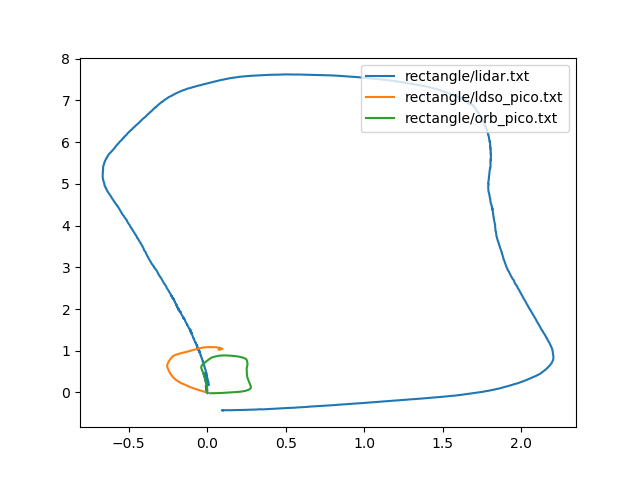
\includegraphics[width=1.0\linewidth]{rectangle1}
		\caption{Trajectory plot without scale factor}
		\label{fig:rectangle1}
	\end{subfigure}
	\begin{subfigure}{.5\textwidth}
		%\centering
		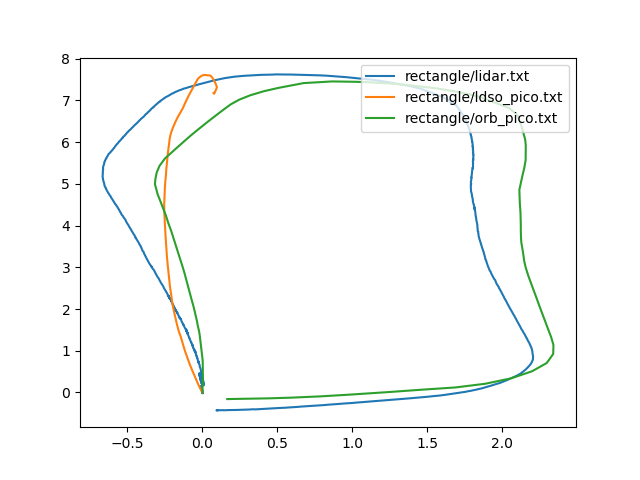
\includegraphics[width=1.0\linewidth]{rectangle2}
		\caption{Trajectory plot with scale factor}
		\label{fig:rectangle2}
	\end{subfigure}
	\caption{Trajectory plots of rectangle path}
	\label{fig:rectangle}
\end{figure}

\section{Observations}
This section covers some observations all \acrshort{vo} which are found during implementation phase. Based on that best algorithm is adopted for further research.
\subsection{\acrshort{svo}}
\acrshort{svo} has main implementation on \acrshort{ros}. Non-\acrshort{ros} version has no visualization functionality which makes it difficult to see what is actually happening. A frame drawer is implemented showing \acrshort{klt} during initialization and \acrshort{fast} features after initialization. \acrshort{svo} is designed mainly for flying robots and due to that its authors have designed it that way. For example, to make it faster (because of drone camera has more FPS than planer robot) and run on \acrshort{cpu} the corner detection is applied only on 3 pyramid levels, number of keyframes at a time are only 3, number of maximum features are 120, smaller grid size of 30. These parameters are not tested in this scope but they can improve result with consequences directly on efficiency. \\
\newline In code implementation, keyframes are selected only if camera travels 15\% of average scene depth while in case of forward facing camera scene depth is always much larger than motion and no new keyframes will be selected. The seeds are updated only in frames which comes after its creation which is only possible in down looking camera because in forward facing camera seeds can be seen in older frames and they won't added to those frames which makes it more difficult to use.

\subsection{\acrshort{ldso}}
\acrshort{ldso} is an extension of \acrshort{dso} with loop-closure using pose-graph optimization. \acrshort{dso} has complex back-end implementation which is not an easy task to modify. Though some parameter modification improved initial results on some straight path but when camera travels in sharp rotation it starts drifting. As authors have already mentioned \cite{yang2018challenges} that without photometric calibration \acrshort{ldso} may not have better performance which is expected because it directly monitors image pixel intensity.\\
\newline It was observed that \acrshort{ldso} gives better performance than \acrshort{orb}-\acrshort{slam} in some cases while using Genius Widecam F100 because it has not accurate intrinsic calibration parameters and \acrshort{ldso} does not depend on feature pixels rather on intensity. \acrshort{ldso} has very high memory usage which makes its no-entry for implementation directly on mobile robot. Which might be due to its complex energy optimization of feature intensity.\\
\newline In texture less environment it can perform better than other methods due to its direct approach. Loop-closure helps it to correctly optimize the previous poses but at cost of high computation. As \acrshort{ldso} uses \acrlong{bow} approach for feature matching and loop closing which is provided by \cite{DboW}. To avoid finding wrong loops parameters are set very strict. It is suggested that a custom \acrlong{bow} vocabulary based on environment should be used which helps to improve performance. Though \acrshort{ldso} uses \acrshort{orb} descriptors but it uses \acrshort{fast} corner detection which might affect the performance. \acrshort{ldso} takes more frames as keyframes than \acrshort{orb}-\acrshort{slam} and further process it which is also a reason for high \acrshort{cpu} load.

\subsection{\acrshort{orb}-\acrshort{slam}}
\acrshort{orb}-\acrshort{slam} is the best performing above all methods in terms of robustness and repeatability. \acrshort{orb}-\acrshort{slam} requires parameter tweaking according to use case and environment. e.g. camera properties, robot velocity, features in environment.\\
\newline  \acrshort{orb}-\acrshort{slam} utilizes much less memory compared to \acrshort{ldso}. Due to that only it could perform the experiment 4 (which has longer run-time) as seen in figure \ref{fig:orb_pico4}. Even without loop closure \acrshort{orb}-\acrshort{slam} shows much less absolute trajectory error as seen in experiment 2 \ref{fig:orb_pico2} and figure \ref{fig:rectangle2}.\\
\newline Though \acrshort{orb}-\acrshort{slam} is robust, it still cannot use directly on mobile robot without any additional sensor which provides absolute scale information. One possible way is to fix camera on looking towards ground and estimating scale based on planer scene assumption provided there is enough features on \acrshort{roi}. During experiments it is noted that whenever there is some motion blur in camera, \acrshort{orb}-\acrshort{slam} cannot track trajectory and always goes in relocalization phase. In this phase it retracks only if it finds some loop closure. In case of Genius Widecam, during rotation \acrshort{orb}-\acrshort{slam} suddenly starts scale drifting as seen in figure \ref{fig:orb_web5} due to motion blur and poor image quality.

\section{Suggestions}
This section outlines some ideas which can be implemented to improve the performance of and real-time applications \acrshort{orb}-\acrshort{slam}.\\
\newline As already mentioned that \acrshort{orb}-\acrshort{slam} has many hard-coded parameters which vary based on applications and camera used. There are still many parameters which can be tweaked to improve accuracy and efficiency both. An extra sensor can be integrated to provide absolute scale information such as \acrshort{imu}, \acrshort{lidar} etc. As proposed by \acrshort{orb}-\acrshort{slam} authors \cite{orbslam} that \acrshort{imu} overcomes the drifting of scale and it can also be used in false loop detection which makes it more preferable to use on real-time applications. During this thesis work a successor of \acrshort{orb}-\acrshort{slam} (version 3) is released which features \acrshort{imu} integration \cite{ORBSLAM3}. \\
\newline To improve speed of \acrshort{orb}-\acrshort{slam} a camera with lower resolution can be used also a custom \acrshort{bow} library is also proven to be faster like one used here \cite{Fbow}. During this thesis lot of work has been done on hardware. There are some camera properties which play an important role in robustness e.g higher \acrshort{fps}, wide \acrshort{fov}, image resolution, exposure time etc. Mobile robot used in this thesis has observed some problems during offline tests when all three sensors (Picocam, Genius Widecam and \acrshort{lidar}) are used together. Genius Widecam can be removed due to its poor performance which will solve the issue (big problem during experiment). \\
\newline A proper ground truth can be prepared for quantitative evaluation. Possible solutions are range finder, an already prepared map of environment, overhead camera tracking a marker on mobile robot. Note that these are possible only in indoor and limited environment.  